\documentclass{paper}

\usepackage{color}
\usepackage{url}
\usepackage{framed}
\usepackage{enumerate}
\usepackage{xcolor,colortbl}
\usepackage{wrapfig}
\usepackage{tabularx}
\usepackage{graphicx}
\usepackage{mathtools}

\usepackage{balance}
\usepackage{multirow}

\usepackage{microtype}
\usepackage{xcolor}

\usepackage{amsmath}
\usepackage{makecell}
\usepackage{colortbl}
\usepackage{xstring}

\usepackage{booktabs}

\PassOptionsToPackage{hyphens}{url}\usepackage{hyperref}

\definecolor{Gray}{gray}{0.85}
\newcommand{\mytablesize}{\scriptsize}
\newcommand{\note}[1]{\textbf{\sf [\underline{SJ}: {\color{red}#1}]}}

\newenvironment{myquote}
{\definecolor{shadecolor}{rgb}{0.9,0.95,1} \begin{shaded*} \sf \em}
{\em\end{shaded*}}

\newenvironment{myquoteOrange}
{\definecolor{shadecolor}{rgb}{1,0.9,0.83} \begin{shaded*} \sf \em}
{\em\end{shaded*}}

\oddsidemargin = -0pt
\topmargin = 0pt
%\textheight = 690pt
\textwidth = 460pt


\newcommand{\sj}[1]{\textcolor{red}{Sagar: #1}}
\newcommand{\la}[1]{\textcolor{blue}{Luca: #1}}
\newcommand{\dq}[1]{\textcolor{green}{Daniele: #1}}

\begin{document}

%\begin{quote}
%{\bf \Large ``} quote here.~{\bf \Large ''}
%\end{quote}

%\begin{myquoteOrange}

\title{Response to the reviews for Royal Society Open Science submission ``FaceLift: A transparent deep learning framework to beautify urban scenes''}
\author{\small Sagar Joglekar, Daniele Quercia, Miriam Redi, Luca Aiello, Tobias Kauer, Nishanth Sastry}
\maketitle

We would like to express our sincere thanks to the Editors for supporting this process and the reviewers for their very detailed and constructive comments. We have worked to address all their concerns in the revised version of the manuscript.
%Below, we first provide a summary of our major changes, followed by a detailed response to each comment of every reviewer.

\section*{Summary of reviewer requests}

\begin{myquote}

\noindent Reviewers made certain important points which we try to address in this revision:

\begin{enumerate}
\item Reviewer 1 expressed concern about the validity of the ``Walkability'' metric actually quantifying walkability of places
\item Reviewer 1 expressed concern about the validity of the ``Openness'' metric actually quantifying open nature of places. They also suggested trying out Scene Understanding (SUN) attributes from places 205 to address this. 
\item Reviewer 2 recommended adding definition for urban informatics along with a reference.
\item Reviewer 2 recommended discussion the PlacePulse dataset in more detail. `` how it was created, and who participated in the curation and assignment of labels. What biases are present in this dataset? Has this been analysed?''
\item Reviewer 2: Looking at the representative examples in Table 4, the ``mechanism'' or trained logic of the algorithm seems quite straightforward, as acknowledged by the authors, e.g. ``adding greenery, narrow roads, and pavements.'' However, I also note that images in rows 3 and 4 shift from a winter scene (trees with no leaves) to a summer scene, or a grey sky to a blue sky. Further, some suggested beautifications shift entire structures such as buildings. These observations could be discussed, and then used to talk about two points: (a) limitations of the approach, and; (b) usefulness of the results (beyond what is covered in Q4). 
\item Reviewer 2: Section Q4 did not convince me. The Likert scale sought to evaluate how well FaceLift supports decision making. It is not clear to me what is meant by decision making here. Similarly, I do not see how the substitution of an act of human creativity through a deep learning algorithm can be rated as "participatory urbanism" when there is nobody participating other than the machine. 
\item Reviewer 2 recommended adding critical reflections about the framework and have kindly given pointers to do so.
\end{enumerate}

\end{myquote}

\noindent We have thoroughly revised the paper to address all the comments from the reviewers. Below, we provide detailed answers to each of their comments individually. In the revised manuscript, changes are highlighted in \textcolor{blue}{blue}.

%\begin{enumerate}

%\item We discussed the Reviewer 1's concern about Walkability as a part of our limitations section. Indeed we believe that the method of quantifying walkability could actually quantify some other abstract quality akin to, but not exactly, ``walkability''. To further help with reflection upon the notion of walkability in this paper's context, we added a table of categorization of PlacesNet labels into 'Natural' , 'Walkable' , 'Architectural' and 'Landmark categories'

%\item We have addressed Reviewer 1's concern about openness by explaining our choice of method to measure openness. To further bolster the argument, we experimented with Scene Understanding framework as suggested. We observe that indeed the attributes further validate some of our findings, are not suitable in measuring the relationship between openness and beauty.

%\item We further clarify other questions by reviewer 1 by adding the necessary text in the paper. 

%\end{enumerate}

%A detailed breakdown of the actions taken can be found next.

\section*{Requests from Reviewer 1}
\begin{myquote}
    First of all, is there a full list of all the keywords used for each metric? This would be a useful addition to a Supplementary Information section. For ``Walkability'', I am concerned that the categories chosen (e.g. plaza, courtyard, park) tend to be places that people go to rest rather than walk. So I am undertrain(sic) that these categories are measuring something akin to walkability of a scene – they might be measuring something else entirely. This might still be a good urban design metric, but I am just not convinced it is measuring walkability. 
\end{myquote}

To classify the PlacesNet labels into the Walkable category, we rely on the definitions of Walkable areas from previous work~\cite{quercia2015digital}, which uses 8 properties of streets to score their walkability: \textit{Road safety, Easy to cross, Sidewalks, Hilliness, Navigation, Safety from crime, Smart and beautiful, Fun and relaxing}. We use these 8 properties as a guidance to classify the PlacesNet labels into the Walkable category. We summarize this categorization in a new Table (see the bottom of this letter and Table 6 in the new manuscript). The elements in the Walkable category serve different functions but they are all either walkable spaces or they are most often situated in walkable areas. We do agree with the Reviewer that walkability acts often as an enabler for other desirable properties of places---like their restorative potential---and therefore it is confounded with them. In the new version of the manuscript, in Section ``Q2 Are beautified scenes great urban spaces?,'' we acknowledge that our walkability measure could correlate with the notion of beauty because it might also act as a proxy for higher-order properties that are enabled by walkability:

\begin{quote}
{\bf \Large ``}~We manually select only the PlacesNet labels that are related to walkability, using a list walkability properties of streets that have been defined in previous work as a guidance~\cite{quercia2015digital}. These labels include, for example, abbey, plaza, courtyard, garden, picnic area, and park (Table 6 contains the exhaustive list) [...] Unsurprisingly, beautified scenes tend to show gardens, yards, and small paths. By contrast, uglified ones tend to show built environment features such as shop fronts and broad roads. It is worth noting that walkability often acts as an enabler for other desirable properties of places (e.g., their restorative capability). The reason why our walkability measure correlates with beauty might be because walkability acts as a proxy for such higher-order properties.~{\bf \Large ''}
\end{quote}

%Indeed there is a real possibility that our method of quantifying walkability could be actually quantifying some other abstract quality akin to, but not exactly, ``walkability''. To that end we discussed the Reviewer's concern about Walkability as a part of our limitations section.

%\begin{quote}
%{\bf \Large ``}~
%Another important limitation is the possibility that our metrics are not actually capturing urban metrics like ``Walkability'' and ``Openness''. It is possible that the PlacesNet~\cite{zhou2014learning} labels could actually be capturing something akin to walkability. We try to reduce this risk by using definitions found in the literature~\cite{quercia15thedigital,ewing2013measuring} as a guidance to classify the PlacesNet labels into the 4 categories
%~{\bf \Large ''}
%\end{quote}

%To reflect upon this, we add a table (see the bottom of this letter and Table 8 in the paper) as a part of our supplementary material. This table lists all the 4 categories into which the placesNet labels are classified. 


\begin{myquote}
    As for ``Privacy-Openness'' – I am not convinced by the approach used to measure openness of a scene. Where a scene with tall trees would feel cozy, a scene with tall skyscrapers is likely to feel claustrophobic rather than cozy. So I am not convinced that lower sky presence equates to coziness, as this really depends on context. It is possible to extract Scene UNderstanding (SUN) Scene Attributes from Places205. These include elements such as far-away horizon, nohorizon, open area; perhaps this could be a helpful way of measuring the ``Privacy-Openness'' aspect of a scene. 
\end{myquote}

\noindent We counted the amount of ``sky pixels'' to measure openness because we wanted to characterize this property on a continuous spectrum, which is not possible with other frameworks. Also, as we will discuss next, the Scene UNderstanding (SUN)~\cite{patterson2012sun,zhou2016places} framework does not have a direct way to quantify the amount of visible sky. However, we followed the Reviewer's suggestion and conducted an additional experiment using SUN.

\noindent We first extracted scene attributes from all the beautified and uglified scenes using SUN, so that each scene gets assigned a list of attributes. Within each group, we counted the number of pictures with a given SUN attribute $i$. We denote these counts as $\phi_i^{beauty}$ and $\phi_i^{ugly}$. We then calculated the differences of these counts between the two groups: $\Delta(\phi_i) = \phi_i^{beauty} - \phi_i^{ugly}$. Figure~\ref{fig:SUN} in this letter shows the distribution of these differences. Positive (negative) values indicate that the attribute is more prevalent in the beautified (uglified) group. Scene attributes like \textit{trees}, and \textit{foliage} are found more frequently in beautified scenes, whereas attributes like \textit{man-made, driving}, and \textit{no horizon} are found predominantly in uglified scenes. These results partially confirm our findings, in that they reveal the broad distinction between beautiful environments with natural elements vs. places where only man-made elements are visible. 

\noindent Categories like \textit{open area}, \textit{enclosed area}, and \textit{no horizon} do not necessarily reflect the amount of visible sky, as it is shown in the discussion from the original paper~\cite{patterson2012sun}. For example, \textit{open areas} represents outdoor places but include both open-sky scenes as well scenes where sky is occluded by trees. Similarly, \textit{enclosed areas} depict walled constructions that might be in areas with different exposure to open sky.

%This corroborates the hypothesis that the lack of horizon or enclosed spaces (lack of openness in general) are not conducive to the feeling of beauty. 

\noindent In short, SUN provides some support to our findings but its results cannot provide a direct measure of openness. The reviewer is right in noting that, in general, lack of openness could indicate cozyness as well as visual oppression. In our specific dataset, spaces with more visible sky tend, on average, to be less visually appealing. We did not add these additional results in the paper, but if the Reviewer thinks it would be useful to have them in the camera-ready version, we will be happy to include them.


%thta said, this is not a perfect predictor, and there will be places with restricted sky view that are ugly.

%To test our hypothesis about the relationship of perceived urban beauty with openness, we needed a metric that could be varied continuously to obtain a progressive trend (As seen from Figure 8.b). The amount of ``Sky'' pixels in an image allowed us to measure a fraction, which can be investigated across the population on a continuous scale. But the metric of openness is a challenging metric to validate.

%Hence to further bolster our insights, we incorporated the suggestion about Scene Understanding Attributes. As per the suggestion we conducted an additional experiment with the Scene Understanding framework~\cite{zhou2016places}. We first extracted scene attributes from all the beautified and uglified scenes. This resulted in a list of scene attributes for the beautified (which we call $\phi_{beauty}$) and a list for the uglified (which we call $\phi_{ugly}$). We then calculated the difference between frequencies of each scene attribute among  $\phi_{beauty}$ and $\phi_{ugly}$. Figure \ref{fig:SUN} shows these differences. A positive difference implies that the attribute is more prevalent in $\phi_{beauty}$) and a negative difference implies that the attribute is more prevalent in $\phi_{ugly}$. Indeed as seen from Figure \ref{fig:SUN}, we observe that scene attributes like \textit{trees, foliage, open area, vegetation, grass} are found in more numbers in beautified scenes. On the contrary, attributes like \textit{man-made, driving, no horizon , far-away horizon, enclosed-area} are found in more numbers in the uglified scenes. This validates the hypothesis that the lack of horizon or enclosed spaces (lack of openness in general) are not conducive to the feeling of beauty. However, it does not give us the flexibility needed in investigating a continuous trend in variation of openness, due to the discrete nature of the scene attributes.

%\begin{quote}
%{\bf \Large ``}~
%~{\bf \Large ''}
%\end{quote} 

\begin{figure}[!htb]
    \centering
    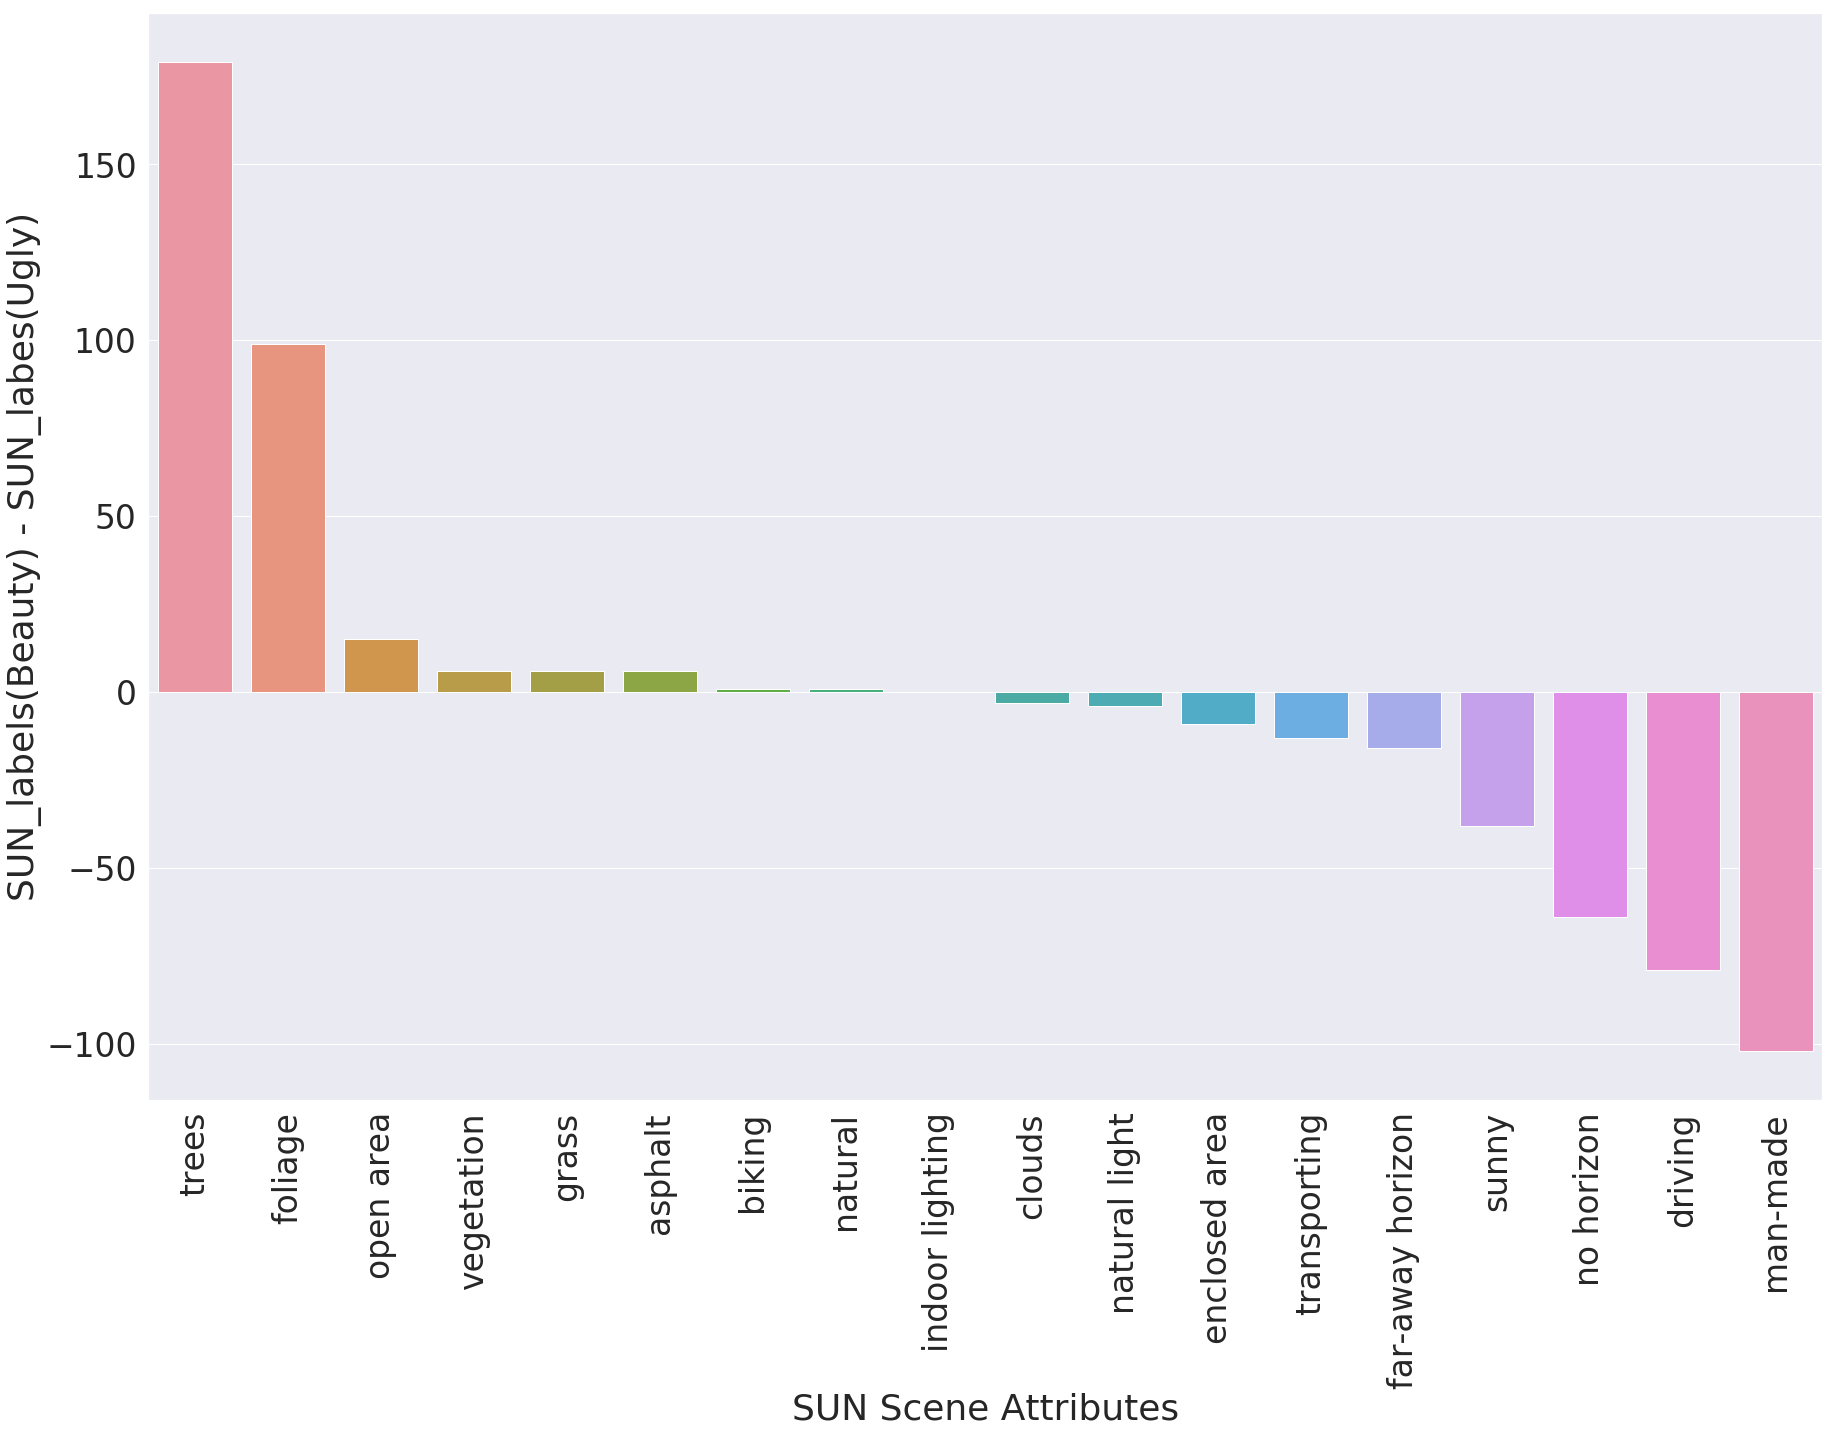
\includegraphics[width=\columnwidth]{figs/SUN.png}
    \caption{}
    \label{fig:SUN}
\end{figure}

\begin{myquote}
    Also note some small changes: 
    \begin{itemize}
        \item - How is similarity calculated on page 4? Is this cosine similarity? 
        \item - It would be useful to add citations to support p.14 ``previous literature''
     \end{itemize}
\end{myquote}

\noindent We used Euclidean distance and we made sure to mention it in the revised version in page 4 (step 4). In page 14, we added 5 citations that cover the ``previous literature'' we refer to.

%We discuss the distance metric used for the retrieval on page 9 \textbf{Step 4 Returning a realistic beautiful scene}. However to address this comment, we added text on page 4 in step 4 
%    \begin{myquoteOrange}
%    ``We use the euclidean distance the compute similarity''
%    \end{myquoteOrange}
%We discuss the expected trends around the 4 metrics based on literature in Table 5. But in addition we have added the necessary references on page 14


\section*{Requests from Reviewer 2}

\begin{myquote}
    The paper specifies and explains key terms such as urban design, deep learning, and generative models, but not urban informatics. Perhaps add a definition and reference. 
\end{myquote}

\noindent As suggested by the reviewer, in the introduction we added a definition for ``urban informatics'' together with a couple of supporting references:

\begin{quote}
{\bf \Large ``}Our work contributes to the field of urban informatics, an interdisciplinary area of research that studies practices and experiences across urban contexts and creates new digital tools to improve those experiences~\cite{foth2009handbook,foth2011urban}.~{\bf \Large ''}
\end{quote}


\begin{myquote}
    It would be useful for the reader to better understand the Place Pulse dataset, how it was created, and who participated in the curation and assignment of labels. What biases are present in this dataset? Has this been analysed? ...
\end{myquote}
%
%The PlacePulse~\cite{dubey2016deep} was acquired through crowd sourced votes on comparisons between two street-view images at a time. The dataset contains google streetview images from 56 major cities across 28 countries. In all the dataset contains more than 1.2 million pairwise votes on 110k images, given by 82k online volunteer voters. The original paper claims that the participant's votes were not influenced by their age, gender or location, which signifies insignificant cultural bias. In addition to the existing dataset description, we added the following text to the paper (page 4) according to the reviewer's suggestion 
%
\noindent We agree with the reviewer that a more self-contained description of the Place Pulse dataset and of its potential biases is in order. We added the following paragraph in the Section ``Curating Urban Scenes'' (page 4):

\begin{quote}
{\bf \Large ``}~To begin with, we need highly curated training data with labels reflecting urban beauty. We start with the Place Pulse dataset that contains a set of 110k Google street view images from 56 major cities across 28 countries around the world~\cite{dubey2016deep}. The pictures were labeled by volunteers through an ad-hoc crowdsourcing website\footnote{\url{http://pulse.media.mit.edu}}. Volunteers were shown random pairs of images and asked to select which scene looked more beautiful, safe, lively, boring, wealthy, and depressing. At the time of writing, 1.2 million pairwise comparisons were generated by 82k online volunteers from 162 countries, with a good mix of people residing in both developed and developing countries. To our knowledge, no independent systematic analysis of the biases of Place Pulse has been conducted yet. However, it is reasonable to expect that representation biases are minimized by the substantial size of the dataset, the wide variety of places represented, and the diversity of gender, racial, and cultural background of the raters.~{\bf \Large ''}
\end{quote}

%\begin{myquoteOrange}
%    The labelling was performed by more than 82k online volunteers. The authors claim that the voting patterns exhibited no significant cultural bias.
%\end{myquoteOrange} 

\begin{myquote}
    Looking at the representative examples in Table 4, the ``mechanism'' or trained logic of the algorithm seems quite straightforward, as acknowledged by the authors, e.g. ``adding greenery, narrow roads, and pavements.'' However, I also note that images in rows 3 and 4 shift from a winter scene (trees with no leaves) to a summer scene, or a grey sky to a blue sky. Further, some suggested beautifications shift entire structures such as buildings. These observations could be discussed, and then used to talk about two points: (a) limitations of the approach, and; (b) usefulness of the results (beyond what is covered in Q4).
\end{myquote}

We agree with the reviewer that the examples in Table 4 expose some of the limitations of our approach. These can be broadly summarized by saying that generative image models are still hard to control, especially when dealing with complex scenes with several elements. This shortcoming is compounded by the restricted size of training data. We briefly mentioned this limitation in the previous version of the paper; in the new manuscript, we expand on that point:

\begin{quote}
{\bf \Large ``}~The main limitation is that generative image models are still hard to control, especially when dealing with complex scenes containing multiple elements. Some of the beautifications suggested by our tool modify the scenes too dramatically (e.g., shifting buildings or broadening roads) to use them as blueprints for urban interventions. This undesired effect is compounded by the restricted size and potential biases of the data that we use both for training and for selecting the scene most similar to the machine-generated image---which might result for example in generating scenes set in seasons or weather conditions that differ from the input image. To address these limitations, more work has to go into offering principled ways of fine-tuning the generative process, as well as into collecting reliable ground truth data on human perceptions. This data should ideally be stratified according to the people's characteristics that impact their perceptions.~{\bf \Large ''}
\end{quote}

Even though this limitation partly restricts the capacity of our tool, we still argue for its potential to simplify and democratize the process of creating restorative spaces, as we detail in the next reply.

\begin{myquote}
    Section Q4 did not convince me. The Likert scale sought to evaluate how well FaceLift supports decision making. It is not clear to me what is meant by decision making here. Similarly, I do not see how the substitution of an act of human creativity through a deep learning algorithm can be rated as ``participatory urbanism'' when there is nobody participating other than the machine.
\end{myquote}

We thank the Reviewer for allowing us to clarify this point, as we realize we could be clearer on the purpose for which FaceLift is intended. We added the following discussion in the conclusions section, hoping that it will serve to clarify the intended use cases for our tool:

\begin{quote}
{\bf \Large ``}~We conceived FaceLift not as a technology to \emph{replace} the decision making process of planners and architects, but rather as a tool to \emph{support} their work. Facelift could integrate the creative process of beautification of a city by suggesting imagined versions of what urban spaces could become after applying certain sets of interventions. We do not expect machine-generated scenes to equal the quality of designs done by experts. However, unlike the work of an expert, Facelift is able to generate beautified scenes  very fast (in seconds) and at scale (for an entire city), while quickly providing a numerical estimate of how much some urban elements should change to increase beauty. The user study we conducted suggests that these features make it possible to inspire the work of decision makers and to nudge then into considering alternative approaches to urban interventions that might not otherwise be apparent. We believe this source of inspiration could advantage non-experts too, for example by helping residents to imagine a possible future for their cities and by motivating citizen action in the deployment micro-interventions.~{\bf \Large ''}
\end{quote}




\begin{myquote}
    This brings me to suggest the addition of a critical reflection and limitations section. Two examples of points that could be explored here: 
    
    (a) The mechanistic/positivist way the algorithm beautifies urban scenes risks becoming a cookie cutter as it does not take into account the full spectrum of authentic ways urban scenes can be activated and then perceived as beautiful. Similarly to how a leafless tree in winter is perceived less beautiful than a lush, leafy tree in summer, there are influences of people, urban policies, placemaking initiatives that impact on the notion of ``beauty.'' Norberg-Schulz (1980) uses a phenomenology approach to describe the ``essence'' of a place, which is socio-culturally and time-specific. Brand (1997) traces the development of a street scene / building façade over time as it changes through renovations, modifications, and customisations and as a result, perceptions change. In my own work (2017), I reviewed placemaking interventions and explored participatory forms of citymaking. 
    \begin{itemize}
    
    \item Norberg-Schulz, C. (1980). Genius loci: Towards a phenomenology of architecture. New York, NY: Rizzoli. 
    
    \item Brand, S. (1997). How Buildings Learn: What Happens After They’re Built (Rev.). London: Phoenix Illustrated. 
    
    \item Foth, M. (2017). Lessons from Urban Guerrilla Placemaking for Smart City Commons. In Proceedings of the 8th International Conference on Communities and Technologies (C\&T '17). ACM, New York, NY, USA, 32-35. DOI: https://doi.org/10.1145/3083671.3083707 
    \end{itemize}
    
    (b) The positivist paradigm of urban science has been critiqued for its technocratic worldview, and the FaceLift study would benefit from a critical reflection by the authors that picks up on some of these points, e.g.: 
		
    \begin{itemize}
    \item Kitchin, R. (2017). Thinking critically about and researching algorithms. Information, Communication and Society, 20(1), 14–29. https://doi.org/10.1080/1369118X.2016.1154087 
    
    \item Dourish, P. (2016). Algorithms and their others: Algorithmic culture in context. Big Data \& Society, 3(2). https://doi.org/10.1177/2053951716665128 
    
    \item Kitchin, R. (2016). The ethics of smart cities and urban science. Philosophical Transactions. Series A, Mathematical, Physical, and Engineering Sciences, 374(2083). https://doi.org/10.1098/rsta.2016.0115 
    
   \end{itemize}
	
\end{myquote}

\noindent We fully agree with these remarks and with the need of emphasizing such limitations and potential risks. We took the suggestion onboard and further expanded our limitations section following what the Reviewer exposed so expertly in their comment.

\begin{quote}
{\bf \Large ``}~There exists a wide spectrum of authentic ways urban scenes could be considered beautiful, because the ``essence'' of a place is socio-culturally and time-specific~\cite{norberg80genius}. The collective perception of the urban environment evolves over time as its appearance and function change~\cite{brand1995buildings} as a result of shifting cultures, new urban policies, and placemaking initiatives~\cite{foth2017lessons}. An undiscerning, mechanistic application of machine learning tools to urban beautification is undesirable because current technology does not take into account most of these crucial aspects. Facelift is no exception, and this is why we envision its use as a way to support new forms of citymaking rather than as a tool to replace traditional approaches. Nevertheless, we emphasize the need of a critical reflection on the implications of deploying such a technology, even when just in support of placemaking activities. In particular, it would be beneficial to study the impact of the transformative effect of Facelift-inspired interventions on the ecosystem of the city~\cite{dourish2016algorithms,kitchin2017thinking} as well as exploring the need to pair its usage with practices and principles that might reduce any potential undesired side effects~\cite{kitchin2016ethics}.~{\bf \Large ''}
\end{quote}

\begin{myquote}
    A suggestion for future work: The Living Building Challenge (LBC) is a performance assessment framework for the built environment that introduces non-traditional and qualitative measures such as beauty. Those buildings and architectural projects that have been assessed by the LBC could perhaps offer a complementary dataset for additional ground truthing from another perspective: https://living-future.org/lbc/beauty-petal/ 
\end{myquote}

\noindent We thank the Reviewer for this relevant pointer. We added a mention to LBC as a possible source of validation data that is orthogonal to what we considered in this work.

\vspace{20pt}

We want to express our sincere thanks to the Editors and to the Reviewers for all the constructive feedback as well as the positive comments above, and hope they will find the new version of the paper much improved.

\begin{table}[htb!]
    \centering
    \begin{tabular}{ |c|c|c|c| }
        \hline
        \textbf{Architectural} & \textbf{Walkable} & \textbf{Landmark} & \textbf{Natural} \\
        \hline
        Apartment building & Abbey & Airport & Badlands\\
        Building Facade & Alley & Amphitheatre & Bamboo Forest\\
        Construction Site & Boardwalk & Amusement Park & Canyon \\
        Courthouse & Botanical Garden & Arch & Coast \\
        Drive way & Corridor & Amphitheatre & Corn field \\
        Door way & Cottage garden & Baseball Field & Creek \\
        Forest road & Courtyard & Basilica & Desert (Sand) \\
        Garbage dump & Crosswalk & Bridge & Field (cultivated)\\
        Golf course & Fairway & Castle & Field (wild)\\
        Highway & Food court & Wind mill & Mountain \\
        Hotel & Forest path & Cathedral & Snowy Mountain \\
        Inn & Formal Garden & Church & Ocean \\
        Ice skating rink & Herb Garden & Dam & Orchard \\
        Motel & Outdoor Market & Dock & Pond \\
        Office building & Nursery & Cemetery & Rainforest \\
        Parking Lot & Patio & Fire station & Rice paddy \\
        Railroad track & Pavilion & Fountain & River \\
        Residential neighbourhood & Picnic area & Gas Station & Rock arch\\
        Restaurant & Playground & Harbour & Sand bar \\
        Runway & Plaza & Hospital & Sea Cliff\\
        School House & Patio & Lighthouse & Ski slope \\
        Skyscraper & Shopfront & Mansion & Sky \\
        Slum & Topiary garden & Mausoleum & Snow field \\
        Supermarket & Tree farm & Pagoda & Swamp \\
        Outdoor swimming pool & Veranda & Palace & Valley \\
        Tower & Vegetable garden  & Racecourse & Wheat field \\
        Water tower & Yard & Ruin & Desert (vegetation) \\
        Wind farm &  & Rope Bridge & \\
        &  & Ski Resort & \\
        &  & Baseball stadium & \\
        &  & Football stadium & \\
        &  & Subway Station & \\
        &  & Train Station & \\
        &  & Temple & \\
        \hline
    \end{tabular}
    \caption{Classification of the Places-net labels into the four categories.}
		\label{tab:PlacesLabels}
\end{table}

\bibliographystyle{abbrv}
\bibliography{letter}

\end{document}
